\documentclass{article}
\usepackage[utf8]{inputenc} %кодировка
\usepackage[T2A]{fontenc}
\usepackage[english,russian]{babel} %русификатор 
\usepackage{mathtools} %библиотека матеши
\usepackage[left=1cm,right=1cm,top=2cm,bottom=2cm,bindingoffset=0cm]{geometry} %изменение отступов на листе
\usepackage{amsmath}
\usepackage{graphicx} %библиотека для графики и картинок
\graphicspath{}
\DeclareGraphicsExtensions{.pdf,.png,.jpg}
\usepackage{subcaption}
\usepackage{pgfplots}
\usepackage{float}

\begin{document}
\begin{center}
    \LaTeX
\end{center}

\pagestyle{plain}

\section*{h/w 10  sentences  using new vocab and grammar.}

\begin{itemize}
    \item I'm going to go to my brother-in-law's on the weekend to play games.
    \item My great-grandfather’s and great-grandmother’s are going to cook a lot of food. I think my stepsister is going to go to them.
    \item The leaves are falling from the trees. I admit autumn is going to come soon. 
    \item My stepsister is making a further project plan in December. (We have a contract)
    \item Immediate family are coming in July and we are going to the sea.
    \item My extended family are arriving in Vnukovo on Sunday and departing from there on Monday. 
    \item My half-sister and I will have Caesar with chicken and an Americano. (The situation in the cafe)
    \item I’ll probably watch this movie about computer influence when I have free time.
    \item I shall see with sibling tomorrow.
    \item Shall we go shopping with you adopted child?
\end{itemize}

\end{document}
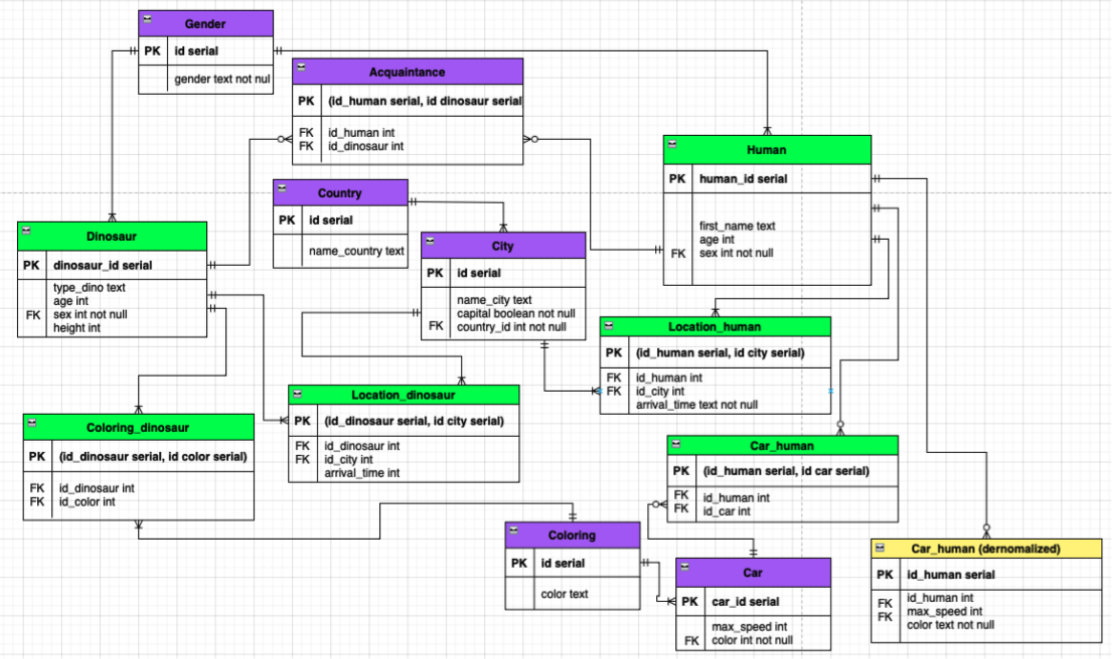
\includegraphics[width=.9\textwidth]{123}